\documentclass[12pt,twoside,a5paper]{amsbook}

\usepackage[usenames,dvipsnames]{color}
\usepackage{epsfig,exscale}
\usepackage[latin1]{inputenc}
\usepackage{hyperref}
 
\usepackage{setspace}
\onehalfspacing

\usepackage[includeheadfoot,
top=20mm,
left=30mm=,
right=20mm,
bottom=15mm
]{geometry}

\renewcommand{\chaptername}{}
\renewcommand{\thechapter}{\Roman{chapter}}
\renewcommand{\contentsname}{�ndice}
\newcommand{\dlg}{\noindent $\bullet$ }

\hypersetup{
pdftitle={Cuentos para ir a dormir},
pdfsubject={cuentos},
pdfauthor={Ariel Narv�ez},
pdfkeywords={cuentos}
}

\title[Cuentos]{CUENTOS PARA IR A DORMIR} 
\author[Ariel Narv�ez]{Ariel Narv�ez}

\begin{document}
\maketitle

\tableofcontents

\chapter{EL COCODRILO Y LAS HORMIGAS}
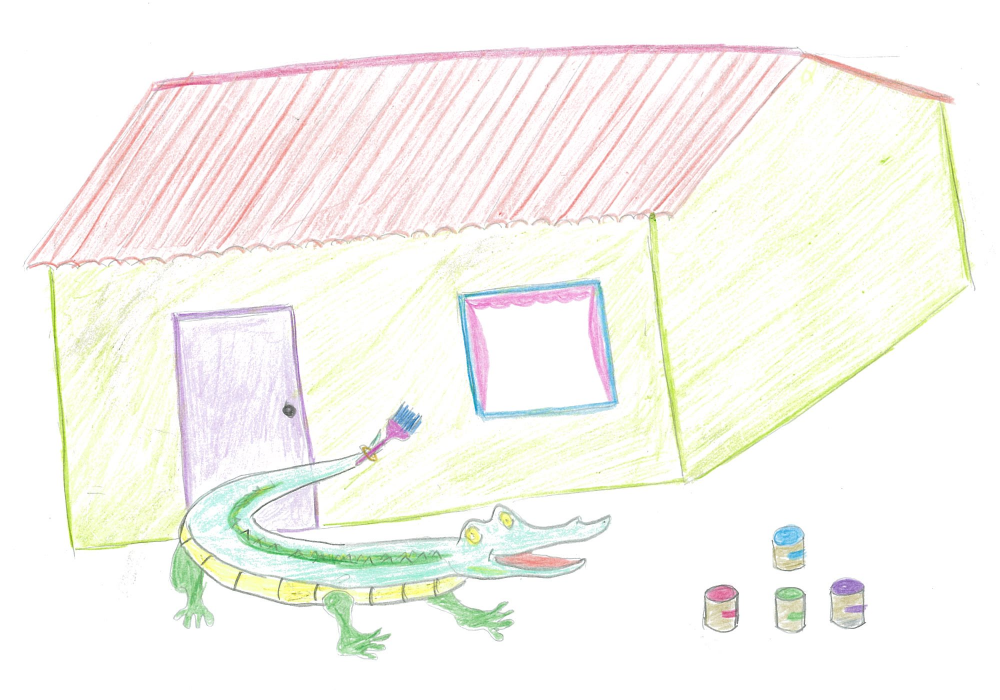
\includegraphics[width=0.8\textwidth]{pics/cocodrilo_1.png}

Un d�a de verano, el cocodrilo como hace varios d�as ten�a ya
preparado, se levant� muy temprano y tras un muy buen desayuno se
dispuso a pintar su casa. Su casa no era muy grande pero ten�a un gran
jard�n con muchas plantas. El cocodrilo ten�a preparado muchas brochas
y todos los colores para las distintas partes de la casa: El techo lo
iba a pintar rojo; las ventanas, azules; la puerta, lila; las paredes,
verdes y la cerca que rodea al jard�n, blanca.

El cocodrilo estuvo pintando sin descanzo durante toda la
ma�ana. Aparte de tomar la brocha sus manos tambi�n utiliz� su cola
para poder as� pintar los rincones dif�ciles de alcanzar. Un poco
antes del medio d�a, el cocodrilo termin� de pintar toda su
casa. Aunque ya ten�a mucha hambre, antes de empezar a cocinar su
almuerzo orden� todos los materiales que utiliz� para pintar. 

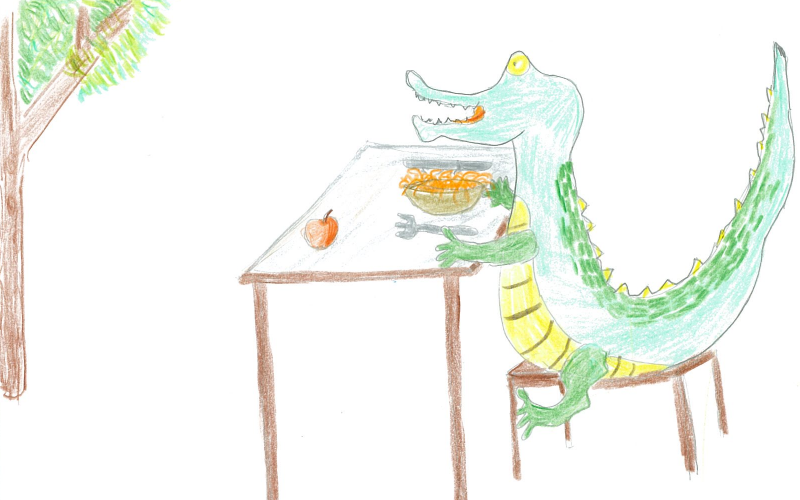
\includegraphics[width=0.8\textwidth]{pics/cocodrilo_2.png}

Su almuerzo consisti� en unos ricos tallarines con salsa y para el
postre ten�a preparada una manzana, pero decidi� ir a descanzar a la
orilla del r�o para luego comer la manzana. En la orilla del rio el
cocodrilo ten�a una mesa y una silla en la cual disfrutaba de tomar
sol en el verano antes de meterse a nadar al r�o. Esta vez no fue la
excepci�n y dej� la manzana sobre la mesa y disfruto del sol en la
silla. Luego de una reponedora siesta, el cocodrilo se meti� al
r�o a nadar. Aunque el r�o ten�a un fuerte caudal, el cocodrilo no
ten�a problemas para nadar con la ayuda de su fuerte cola y con
facilidad cruzaba el r�o de un lado a otro.

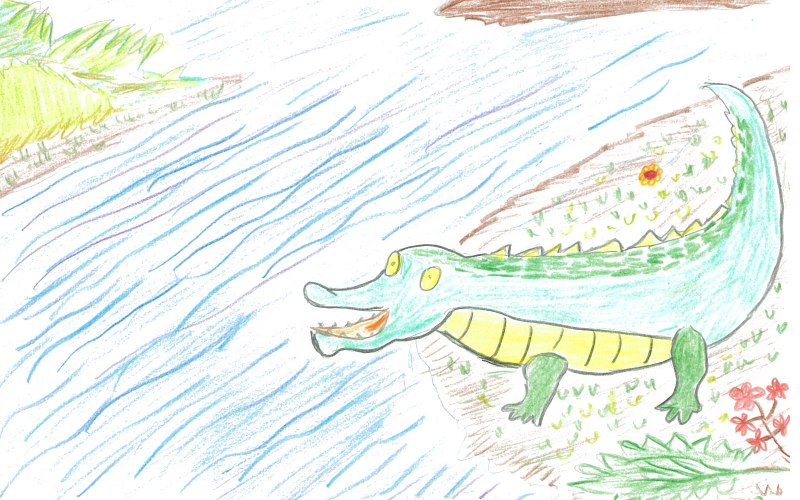
\includegraphics[width=0.8\textwidth]{pics/cocodrilo_3.png}

Al termininar de nadar y disponerse a comer la manzana, el cocodrilo
se encontr� con una sorpresa: la manzana ya no se encontraba sobre la
mesa. El cocodrilo empez� a buscar la manzana, y r�pidamente la
encontr� bajo la mesa, pero algo raro ocurr�a, la manzana lentamente
se mov�a. Al acercarse y mirar detenidamente, el cocodrilo se dio
cuenta que unas hormigas se llevaban su manzana. El cocodrilo les dijo
que le devolvieran su manzana a lo que las hormigas le
res\-pon\-die\-ron: 

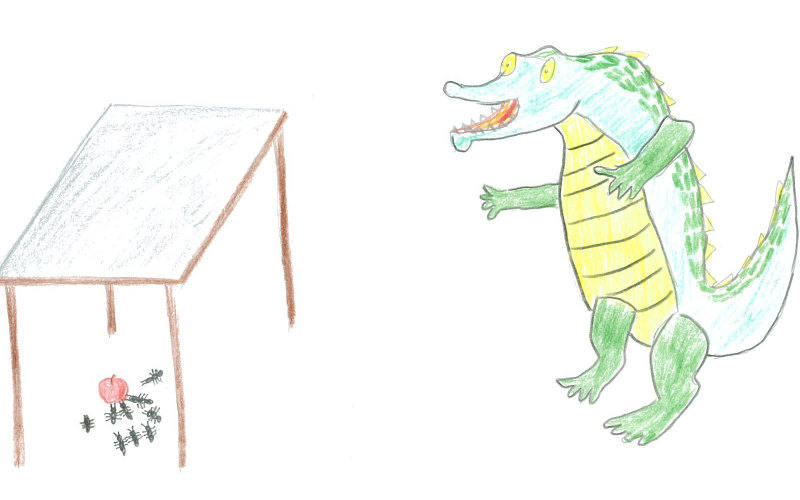
\includegraphics[width=0.8\textwidth]{pics/cocodrilo_4.png}

\dlg  Nosotras somos muchas y tenemos hambre!!! \\
\dlg El cocodrilo muy enojado les dijo: \\
\dlg  si tienen tanta hambre vayan ustedes mismas a buscar
manzanas al �rbol y no me quiten la m�a. \\
\dlg Las hormigas respondieron muy sorprendidas:\\
\dlg  Cu�l �rbol? \\
\dlg Las hormigas no conoc�an el �rbol as� que muy curiosas le
preguntaron al cocodrilo: \\
\dlg  D�nde est� el manzano? \\
\dlg El cocodrilo aunque estaba muy enojado les respondi�
amablemente y les dijo que simplemente ellas ten�an seguir el r�o y
caminar unos 10 minutos y se encontrar�an con el manzano.

Las hormigas le devolvieron la manzana al cocodrilo y partieron
r�pidamente a buscar manzanas. Cuando llegaron al �rbol todas las
hormigas se subieron y sacaron una manzana para cada una.  Adem�s
buscaron la manzana m�s roja y grande del �rbol y se la llevaron de
regalo al cocodrilo para agrecerle por ense�arles la ubicaci�n del
manzano y para pedirle perd�n por tratar de llevarse su manzana.

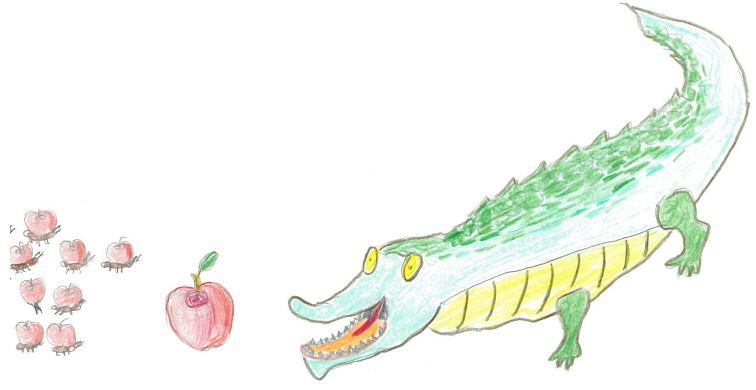
\includegraphics[width=0.8\textwidth]{pics/cocodrilo_5.png}


\chapter{EL LIBRO BENJAMIN}
%\includegraphics[width=0.6\textwidth]{pics/benjamin} 



\chapter{LAS HORMIGAS Y EL TOPO}
Durante todo el verano las Hormigas se fueron a la playa. 
%
Algunas se dedicaron a jugar voleibol, otras al f�tbol, otras a las
paletas, otras a nadar, otras constru�an castillos de arena y las
restantes simplemente disfrutaban del sol.

Cuando el verano acababa, la jefa de las Hormigas llam� a una
reuni�n. La jefa con voz de mando dijo: \\
\dlg Hermanas, nuestras vacaciones en la playa se terminan
hoy. 
%
\fgr{hormigas_1.png}
%
A partir de ma�ana comenzamos la recolecci�n de alimentos para el
duro invierno que viene. 
%
Tenemos dos meses para la recolecci�n y despu�s debemos construir un
hogar para nosotras y nuestra comida.

Todas las Hormigas escuchaban muy atentamente. 
%
La Hormiga secretaria tomaba nota de todo lo que dec�a la jefa.
%
�sta segu�a con su plan: \\
\dlg  Los alimentos necesarios son: trigo, ma�z, arroz, manzanas,
peras, papas, leche, miel, porotos, lentejas y arvejas. 
%
%\fgr{hormigas_2.png}
%
Para eso nos dividiremos en escuadras que se dedicar�n a recolectar
cada uno de estos alimentos. 
%
Mi secretaria ac� tiene la lista con las escuadras.

Para terminar la jefa le dijo al resto de las Hormigas: \\
\dlg Ma�ana comenzamos muy temprano as� que hoy disfruten lo m�s
posible de la playa por que ser� el �ltimo y luego se nos viene un
duro trabajo.

Al d�a siguiente y durante las siguientes semanas las Hormigas
trabajaron sin cesar. 
%
Luego de dos meses de recolecci�n, las Hormigas ya ten�an suficiente
alimentos para el invierno y deb�an ahora iniciar la construcci�n de
su hogar. 
%
Por alguna extra�a raz�n, ese a�o el invierno se adelant� y las
Hormigas a�n no ten�an listo su hogar cuando la nieve ya hab�a
llegado. 
%
Esto era un problema muy grave. 
%
La jefa de las Hormigas les dijo a sus compa�eras: \\
\dlg Debemos encontrar pronto un hogar para nosotras y 
nuestra comida... \\
\noindent En ese momento el Papagayo que miraba desde arriba 
interrumpi� a la jefa y le dijo: \\
\dlg Seg�n lo que yo s�, el Topo agrand� su casa durante el 
verano y tiene, por tal, unas piezas libres que les podr�an 
ser �tiles. 
%
\fgr{hormigas_3.png}
%
Yo ir� r�pidamente a preguntarle.
%
El Papagayo sali� volando r�pidamente y se encontr� con el Topo
explic�ndole el problema de las Hormigas. 
% 
El Topo respondi� r�pida y amablemente: \\
\dlg Ning�n problema, que vengan a vivir conmigo durante el invierno.\\
%
El Papagayo vol� de vuelta y le dio la buena noticia a la Hormigas. 
%
La jefa de la Hormigas r�pidamente organiz� el viaje hasta la casa del
Topo. 
%
Al llegar a la casa del Topo las Hormigas saludaron y agradecieron su
amabilidad.
%
El Topo les respondi�: \\
\dlg Gracias a ustedes que me van a acompa�ar durante el invierno. 
%
Yo vivo solo, trabajo durante todo el d�a afuera y llego muy cansado
en la tarde. 
%
\fgr{hormigas_4.png}

Ese invierno fue muy entretenido para las Hormigas y el Topo. 
%
Las Hormigas usando toda la comida que hab�an recolectado le cocinaban
al Topo una rica cena para cuando �ste llegaba cansado de su trabajo y
despu�s antes de dormir jugaban a las cartas o miraban alguna pel�cula
juntos.





\chapter{EL MENSAJE}
%Muy temprano en la ma�ana, antes que el Gallo cantara, al Dinosaurio,
al Elefante y a la Girafa los despertaron para que
partieran r�pidamente con la misi�n de entregar un mensaje al Le�n.
%
�ste hab�a salido de viaje hace ya casi un mes y por distintos
problemas no hab�a podido regresar aun.

El Dinosaurio, el Elefante y la Girafa no tuvieron tiempo para
preparar nada y salieron r�pidamente con una mochila cargada con un
par de manzanas, unos panes y una botella con agua.
%
Debido a la distancia que se encontraba el le�n, el Dinosaurio, el
Elefante y la Girafa estimaron que les tomar�a todo el d�a caminado
hasta llegar donde el le�n.
%
En el trayecto deb�an cruzar la selva, la sabana y un r�o.
%
Aunque ninguno de los tres sab�a nadar no ten�an miedo del r�o ya que
los tres eran animales muy grandes, por tal, no ser�a necesario nadar
para cruzarlo.

Al poco andar por la selva se encontraron con los chimpanc�s, los cuales
muy ruidosos saludaron.
%
Luego se encontraron con el gorila, que adem�s de saludar les pregunt�: \\
\dlg  Ad�nde van con tanta prisa? \\
El Dinosaurio respondi�:
\dlg Llevamos un mensaje al Le�n, as� que tenemos que caminar 
muy r�pido para llegar antes que oscurezca. \\
\dlg Mucha suerte en su misi�n les dese� entonces. \\
Les dijo el gorila.

Luego de un par de horas caminando, el Dinosaurio, el Elefante y la
Girafa decidieron hacer la primera pausa para comerse las mazanas y
tomar un poco de agua.
%
Retomaron el rumbo y pronto cruzaron la selva y se adentraron en la
sabana.
%
Ac� se encontraron con los ant�lopes y las zebras que muy
cordialmente saludaron.
%
Ya, a la distancia pod�an divisar el r�o y luego de un par de minutos
caminando llegaron a su orilla.
%
El r�o no se ve�a muy profundo pero si con un caudal muy fuerte.
%
El Dinosaurio, el Elefante y la Girafa no ten�an miedo del �ste y se
adentraron en el agua.
%
Al cabo de unos metros sintieron la fuerza del caudal y luego de unos
segundos, cayeron al agua y se fueron por el r�o arrastrados por el
agua.
%
Ninguno de ellos se pod�a poner en pi� nuevamente y rodaban r�o abajo.
%
Por suerte el Cocodrilo que viv�a en el r�o observ� todo lo acontecido
y r�pidamente se met�o al agua y con su fuerte cola avanaz�
r�pidamente, tom� a la Girafa y la cruz� hasta la otra orilla del r�o.
%
Se meti� nuevamente y ahora sac� al Elefante y por �ltimo y sac� al
Dinosaurio.
%
�ste era tan grande que le cost� un esfuerzo enorme arrastrarlo hasta
la otra orilla.

Una vez en la otra orilla, secos, el Cocodrilo les dijo que aunque
ellos eran muy grandes, ten�an que tener cuidado con lo r�os.
%
Muchos no son profundos pero el caudal puede hacer que uno pierda el
equilibrio y se caiga, como les acababa de ocurrir a ellos.
%
Por otra parte, el Dinosaurio, el Elefante y la Girafa se dieron
cuenta que producto de su ca�da al agua, se les hab�a perdido el pan
que tra�an.
%
Ahora ya no ten�an nada m�s para comer y todav�a les quedaba mucho por
caminar.

Caminaron ahora sin descanzo por la sabana, ya se hac�a de noche y
todos los animales se iban a dormir. 
%
El atardecer en la sabana era muy bonito con un sol grande y rojo que
se escond�a en el horizonte acompa�ado de un cielo naranjo.
%
Siguieron su camino y ya hab�an caminado muchas horas en la oscuridad
cuando llegaron donde el Le�n y finalmente pudieron entregarle el
mensaje.
%
El Le�n abri� la carta y pudo leer:
%
\begin{center}
\begin{tabular}{|r|}
\hline
{\sc Tu hijo ha nacido hoy sano y fuerte.} \\
{\sc La Leona.}\\
\hline
\end{tabular}
\end{center}

El Le�n salt� de felicidad y mand� a preparar una gran comida para sus
amigos mensajeros.
%
El Dinosaurio, el Elefante y la Girafa despu�s de un largo d�a
caminando, finalmente pudieron descanzar con el grato sabor de haber
cumplido la misi�n.


\chapter{EL TOPO Y EL MONO}
Luego de un largo invierno, en el cual el Topo se refugi� en su cueva
a dormir, llegaron los primeros d�as c�lidos de
la primavera y, por tal, tiempo de salir de la madriguera.

El Topo, lo primero que hizo fue abrir la entrada de su
madriguera para que entrara luz. 
%
Luego, inspirado por el aire fresco que pudo respirar decidi� limpiar
bien su madriguera ya que durante todo el invierno y mucho polvo se
acumul� en todas partes.

Durante toda la ma�ana el Topo estuvo ocupado en su casa, limpi� las
ventanas, trape� el piso de la cocina y el ba�o, sacudi� los cojines
del sill�n, barri� el piso y luego lo encer�, aspir� la alfombra y
finalmente con el plumero sac� el polvo de los muebles.
%
Con la limpieza a fondo llen� varias bolsas de basura que las dej�
afuera de su casa para ir m�s tarde a botarlas al contenedor.

Luego del arduo trabajo, el Topo estaba listo para descansar. Sali� de
su madriguera y se sent� a la sombra de un �rbol. 
%
Llev� junto con �l una rica sand�a para comer mientras descansaba.

Por otra parte, en la cima de ese mismo �rbol unos minutos antes hab�a
subido el Mono a leer y para comer hab�a llevado un pl�tano.
%
Cuando el Mono se decidi� a comer el pl�tano, lo pel� por completo y
dej� la c�scara colgada de una rama para luego cuando bajara ir a
botarla a la basura.
%
Con una peque�a brisa las ramas del �rbol se movieron y la c�scara
se cay�.
%
El Mono no le dio mayor importancia y se dijo a si mismo que cuando
bajara recoger�a la c�scara y la ir�a a botar a la basura.

La c�scara fue cayendo chocando de rama en rama para finalmente caer
exactamente sobre la cabeza del Topo que descansaba junto con su
sand�a. 
%
El Topo muy enfurecido mir� a todos lados buscando desde d�nde lleg�
la c�scara, no encontr� a nadie, luego mir� hacia arriba y pudo ver al
Mono sentado en la cima del �rbol leyendo un libro y comiendo
pl�tano.
%
El Topo se dijo a si mismo: \\
\dlg Mono cochino, botando las c�scaras en cualquier parte y no 
en el basurero. \\
Luego lo llam�: \\
\dlg \xclm{Mono} \xclm{Mono} \xclm{ven, baja del �rbol} \\
Muy �gil, el Mono baj� del �rbol y salud� al Topo: \\ 
\dlg \prgnt{Qu� pasa Topo} \\ 
El Mono todav�a muy enojado le dice: \\ 
\dlg Mira, la c�scara de pl�tano que tu botaste desde arriba me cay� a
m� en la cabeza. \\
\dlg Esa c�scara yo la dej� sobre una rama para botarla m�s tarde a la
basura y el viento la hizo caer. \\
Le respondi� el Mono. Agregando adem�s: \\
\dlg Mil disculpas amigo Topo, nunca fue mi intenci�n tirar la c�scara 
de pl�tano desde all� arriba. Para que me perdones yo mismo te voy a
ayudar a dejar al contenedor las bolsas de basura que tienes ah�.

El Mono r�pidamente llev� todas las bolsas de basura al contenedor. 
%
Al volver, el Topo le dio al Mono un pedazo de su sand�a mostrando as�
que el malentendido con la c�scara de pl�tano ya estaba superado y
segu�an siendo amigos.




\chapter{LA MANZANA}
Un d�a iban caminando juntos por el campo tres animales muy grandes:
un Elefante, una Girafa y un Dinosaurio. Iban de lo mas felices
conversando cuando se dieron cuenta que en frente de ellos
hab�a un manzano con la �ltima de sus manzanas en el tope de su frondosa
copa.

El primero en decir que la manzana le pertenec�a fue el Elefante, que
dijo de inmediato:\\
\dlg  Esa manzana es m�a, la voy a sacar y me la voy a comer. \\
La Girafa y el Dinosaurio al un�sono replicaron la misma respuesta: \\
\dlg  Yo tambi�n la puedo sacar y me la como.

En resumen, los tres querian la manzana y cada uno estaba muy seguro
que debido a su tama�o no ser�a un problema poder sacala aunque la
manzana en realidad se ubicaba a mucha latura. Luego de discutir el
tema llegaron a un acuerdo: Ser�a la Jirafa la primera en intentar
sacar la manzana, luego vendr�a el Elefante y por �ltimo el Dinosaurio
que era el m�s grande de los tres y de seguro sacar�a la manzana.

La Jirafa se acerc� al �rboly con estir� su largo cuello para poder
alcanzar la manzana. Aun con su mejor esfuerzo, tratando incluso de
pararse s�lo en sus patas traseras, la Jirafa no fue capaz de alcanzar
la manzana. Al darse por vencida, le dio el turno al Elefante. �ste se
acerc� se par� en sus patas traseras y estir� su larga y fuerte trompa
pero no alcanzaba la manzana. Incluso con su trompa intent� zamarrear
las ramas para poder as� botar la manzana. Esto tampoco result�.

Finalmente se acerc� al manzano el Dinosaurio muy seguro de sacar la
manzana, estir� su largo cuello y lo dirigi� haci� la manzana pero
para su sorpresa no la pudo alcanzar. Luego de intentarlo varias veces
se convenci� de que le era imposible.

Los tres m�s grandes animales se encontraban completamente
sorprendidos de que ninguno de ellos fue capaz de sacar la manzana. 

En ese momento se acerca al manzano un peque�o mono que empieza a
escalar y saltar de rama en rama subiendo r�pidamente a la copa del
�rbol. Con la mirada at�nita del Elefante, la Jirafa y el Dinosaurio;
el peque�o mono fue capaz de sacar la manzana y muy feliz bajar del
�rbol comi�ndosela. Los saludo afectuosamente y tan repent�namente
como lleg�, se fue. 

El Elefante, la Jirafa y el Dinasaurio al un�sono se rieron de lo que
hab�a pasado y siguieron su camino.


\chapter{EL GRILLO VIOLINISTA}
Desde ya hace muchas generaciones, la familia del Grillo era conocida
por su m�sica. Por tal, al peque�o Grillo su pap� le ense�o a tocar el
viol�n. As�, cuando �l estuviera viejo, el peque�o Grillo pudiera
heredar su trabajo. El trabajo consist�a en tocar el viol�n todas las
noches y as� ayudar a los animales a dormir.

El tiempo pas� muy r�pido y el pap� Grillo se hizo viejo y no ten�a
las fuerzas necesarias para salir a tocar todas las noches el viol�n.
Para que continuara la tarea el Grillo recibi� de regal� el mejor
viol�n. La rutina era siempre la misma, se iniciaba tocando en el
gallinero para hacer dormir a todas las gallinas y sus pollitos, luego
se iba al chiquero donde se hac�a dormir a todos los chanchos y sus
peque�os lechones. Se contiuaba en el establo donde se hac�a dormir a
los caballos y vacas y a sus peque�os potrillos y terneros. Por �ltimo
se hac�a dormir a las ovejas y se iba a tocar al lado de la ventana de
la pieza donde dormian los hijos del granjero para que �stos tambi�n
tuvieran dulces sue�os.

El Grillo estaba muy feliz de realizar esta linda tarea todos los
d�as, todas las semanas preparabas nuevas canciones para que los
animales durmieran muy bien y pudieran as� poder iniciar el nuevo d�a
llenos de energ�a y del mismo modo para que los peque�os pollitos,
lechones, potrillos, terneros y los hijos del Granjero crecieran
fuertes y sanos. El trabajo del Grillo era muy importante en el campo
y todos los animales le ten�an un gran afecto.

Un d�a el Grillo iba a iniciar su trabajo pero no pod�a encontrar el
viol�n, y sin �l no pod�a salir a tocar. Adem�s ese viol�n era muy
importante para �l por que era el favorito de su pap� y �ste se lo
hab�a regalado. Lo busc� por todas partes y no lo pudo
encontrar. Tanto lo busc� que se hizo tarde, decidi� que ese d�a ya no
saldr�a a tocar y en la ma�ana continuar�a la busqueda. Al otro d�a
muy temprano muchos animales se acercaron a preguntar porqu� no hab�a
tocado la noche anterior. Al explicarles el Grillo, los animales se
sumaron a la busqueda del viol�n.

Pasaron cuatro d�as y el viol�n no aparec�a, muchos animales se ve�an
muy cansados, necesitaban de la m�sica del Grillo para poder dormir
bien y as� reponer las energ�as. En la granja no se hablaba de otro
tema, todos los animales estaban muy preocupados y se organizaron para
todos iniciar una busqueda en todas partes hasta encontrar el viol�n,
la cual denominaron: {\sl Operaci�n Rastrillo}.

Iniciaron la busqueda en el gallinero, revizaron todos los rincones,
luego fueron al chiquero, que era el lugar donde viv�an los chanchos y
estaba muy desordenado pero no encontraron el viol�n. Luego al igual
que la rutina del Grillo todas las noches, todos los animales, fueron
al establo y revizaron en todas partes. Para finalizar fueron a la
casa del Grillo y buscaron sin �xito. Para finalizar se reunieron
todos los animales en el centro del patio. En ese momento lleg� el
Granjero con el viol�n en sus manos, �l lo hab�a tomado y llevado a la
ciudad para que lo restauraran con un nuevo barniz adem�s de
colocarles cuerdas nuevas. Todos los animales saltaron de alegr�a al
ver nuevamente el viol�n, especialmente el Grillo debido a que �ste
era un regalo especial de su Pap�.

Ese d�a el Grillo toc� su mejores canciones y todos los animales
durmieron profundamente.





\end{document}

